% Template for ICME-2013 paper; to be used with:
%          spconf.sty  - ICASSP/ICIP LaTeX style file, and
%          IEEEbib.bst - IEEE bibliography style file.
% --------------------------------------------------------------------------
\documentclass{article}
\usepackage{spconf,amsmath,epsfig}

\usepackage[utf8]{inputenc}

\usepackage{subfig}
\usepackage{enumerate}

% autoref command
\usepackage[hyphens]{url}
\usepackage[pdftex,urlcolor=black,colorlinks=true,linkcolor=black,citecolor=black]{hyperref}
\def\sectionautorefname{Section}
\def\subsectionautorefname{Subsection}
\def\subfigureautorefname{Subfigure}

% listings and Verbatim environment
\usepackage{fancyvrb}
\usepackage{relsize}
\usepackage{listings}
\usepackage{verbatim}
\newcommand{\defaultlistingsize}{\fontsize{8pt}{9.5pt}}
\newcommand{\inlinelistingsize}{\fontsize{8pt}{11pt}}
\newcommand{\smalllistingsize}{\fontsize{7.5pt}{9.5pt}}
\newcommand{\listingsize}{\defaultlistingsize}
\RecustomVerbatimCommand{\Verb}{Verb}{fontsize=\inlinelistingsize}
\RecustomVerbatimEnvironment{Verbatim}{Verbatim}{fontsize=\defaultlistingsize}
\lstset{frame=lines,captionpos=b,numberbychapter=false,escapechar=§,
        aboveskip=2em,belowskip=1em,abovecaptionskip=0.5em,belowcaptionskip=0.5em,
        framexbottommargin=-1em,basicstyle=\ttfamily\listingsize\selectfont}

\pagestyle{empty}

\begin{document}\sloppy

% for 1st, 2nd, etc. superscripting
\newcommand{\ts}{\textsuperscript}

% Title.
% ------
\title{Tell me why! Ain't nothin' but a mistake?\\ Describing Media Item Differences with Media Fragments URI}
%
% Single address.
% ---------------
\name{Anonymous ICME submission}
\address{}

\maketitle

%
\begin{abstract}
We have developed a~tile-wise histogram-based
media item deduplication and clustering algorithm
with additional high-level semantic matching criteria
that is tailored to photos and videos stemming from multiple social networks.
In this paper, we investigate whether the addressing scheme
Media Fragments  {\sc uri} provides a~feasible and practicable way
to vividly and graphically describe media item differences
between media items of type photo and/or video.
\end{abstract}
%
\begin{keywords}
Media Fragments {\sc uri}, Media Fragments, Media Items, Deduplication, Social Networks
\end{keywords}
%
\section{Introduction}
\label{sec:introduction}

The \emph{Backstreet Boys}~({\sc bsb}) are a~boy band
formed in~1993 in Orlando,~FL
that has sold over 130~million records worldwide,
making them the best-selling boy band of all time.
In~2013, the band will celebrate their 20\ts{th}~anniversary
with a~new album and a~world tour.
Reason enough for us to make them titular saint of this paper
with their hit song \emph{I~Want It That Way}
from the album \emph{Millennium}.
While the spike of their career was in the late 90s,
even today, people still actively share,%
\footnote{{\sc bsb} on social networks: \url{http://bit.ly/backstreet-gplus}
and \url{http://bit.ly/backstreet-fb},
both accessed 03/04/2013}
publish, and follow the group on \emph{social networks}.

\subsection{Previous Work}
\label{sec:previous-work}

Social networks are at the heart of our research on event summarization,
specifically deduplicating \emph{exact-} and \emph{near-duplicate}
media items that optionally accompany textual status messages
referred to as \emph{microposts} on multiple social networks. 
In the context of our research, we define a~\emph{media item}
as either a~photo (image) or video
that was \emph{publicly} shared or published
on at least one social network.
\autoref{fig:near-duplicate} shows an example
where two users of the social networks Facebook and Google+
independently of each other share a~\emph{near-duplicate} media item
in form of the music video \emph{Everybody}
performed by the \emph{Backstreet Boys}.
In order to detect, deduplicate, and cluster such occurrences
of \emph{exact-} and \emph{near-duplicate}
media items being shared independently across social networks,
we have implemented a~tile-wise histogram-based algorithm
with additional high-level semantic matching criteria
that was shown to work effectively and efficiently for several events.

\begin{figure}[b!]
  \centering
  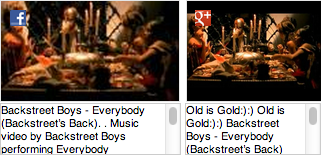
\includegraphics[width=0.75\linewidth]{./backstreetboys.png}
  \caption{\emph{Near-duplicate} music video \emph{Everybody}
    by the \emph{Backstreet Boys} shared
    independently on Facebook and Google+}
  \label{fig:near-duplicate}
\end{figure}

\subsection{Motivation and Research Question}
\label{sec:motivation-and-research-question}

During previous experiments on clustering event-related media items,
we noticed that human raters wanted to know \emph{why}%
\footnote{Tell me why! Ain't nothin' but a mistake?}
certain media items were clustered as \emph{exact-} or \emph{near-duplicates}.
In consequence, in this paper, we investigate in how far
Media Fragments {\sc uri}~\cite{troncy2012mediafragments}
provides a~feasible and practicable way
to tell raters why media items were clustered.
As we deal with media items of type photo and/or video,
we make simultaneous use of two types of media fragment dimensions,
the temporal dimension and the spatial dimension.

\subsection{Paper Structure}
\label{sec:paper-structure}

The remainder of this paper is structured as follows.
In \autoref{sec:related-work}, we report on related work
on media fragments and digital storytelling.
In \autoref{sec:media-item-deduplication-algorithm},
we describe the tile-wise histogram-based
media item deduplication and clustering algorithm.
In \autoref{sec:media-fragment-requirements}, we describe
our requirements on media fragment identifiers.

\section{Related Work}
\label{sec:related-work}

\noindent \textit{Media Fragments:}
Media Fragments {\sc uri}~\cite{troncy2012mediafragments} specifies
the syntax for constructing media fragment {\sc uri}s
and explains how to handle them
when used over the {\sc http} protocol~\cite{fielding1999http}.
The syntax is based on the specification of particular name-value pairs
that can be used in {\sc uri} fragment and {\sc uri} query requests
to restrict a~media resource to a~certain fragment.
Currently supported media fragment {\sc uri}s in the basic version
cover the temporal and the spatial dimension.
The temporal dimension denotes a~specific time range in the original media,
such as ``starting at second 10, continuing until second 20.''
The spatial dimension denotes a~specific range of pixels in the original media,
such as ``a~rectangle of size $ 100 \times 100 $
with its top-left at the coordinates $ (10, 10) $,''
where combinations of both dimensions are possible.

\noindent \textit{Digital Storytelling:}
Pizzi and Cavazza report in~\cite{pizzi2008debugging} on the development of
an authoring technology on top of an interactive storytelling system
that originated as a~debugging%
\footnote{Note, Pizzi and Cavazza use the term \emph{debugging} in the non-IT sense:
to check for redundancy, dead-ends, consistency, \emph{etc.} in authored stories}
tool for a~planning system.
Alexander and Levine define in~\cite{alexander2008storytelling}
the term \emph{Web~2.0 storytelling}, where people create \emph{microcontent}---%
small chunks of content, with each chunk conveying a primary idea or concept---%
that gets combined with social media to form coherent stories.
We use Media Fragments {\sc uri}s to help raters understand
the results of an algorithm by converting dry software debugging data
to digital stories.

\section{Media Item Deduplication Algorithm}
\label{sec:media-item-deduplication-algorithm}

Our near-duplicate media item clustering algorithm belongs to the family of
tile-wise histogram-based clustering algorithms.
As an additional semantic feature, the algorithm considers detected faces.
It is capable of deduplicating both media items of type video and photo.
In the case of video, frames at camera shot boundaries are used. % insert citation
For two media items to be clustered,
the following conditions have to be fulfilled.

\begin{enumerate}
  \item Out of $m$ tiles of a~media item with $n$ tiles ($m \leq n$),
    at most $\textit{tiles\_threshold}$ tiles may differ not more than $\textit{similarity\_threshold}$
    from their counterpart~tiles.
  \item The numbers $f_1$ and $f_2$ of detected faces in both media items
    have to be the same.
    We note that we do not \emph{recognize} faces, but only \emph{detect} them.
\end{enumerate}

In order to illustrate the way the algorithm deduplicates media items,
\autoref{fig:algorithmdebug} shows a~debug view of the algorithm
for the two clustered media items related to the previous example around the
\emph{Backstreet Boys} music video from \autoref{fig:near-duplicate}.
Independent of the actual media item's aspect ratio,
the tile-wise comparison always happens based on a~potentially squeezed
square aspect ratio version.

\begin{figure}[b!]
  \centering
  \subfloat[From Facebook user]{
    
\includegraphics[width=0.3\linewidth]{debug1.png}
  }                
  \subfloat[From Google+ user]{
    
\includegraphics[width=0.3\linewidth]{debug2.png}
  }
  \caption{Debug view of the media item deduplication algorithm
    (as in the concrete case no faces were detected,
    the match happens solely based on tile similarity)}
  \label{fig:algorithmdebug}  
\end{figure}

\section{Media Fragment Requirements}
\label{sec:media-fragment-requirements}

In the context of our research on media item deduplication,
a~media fragment identifier needs to be capable of expressing the following concepts.

\begin{enumerate}[i]
  \item Given a~rectangular media item with the dimensions $ width \times height $,
    express that in turn rectangular tiles
    of smaller dimensions are part of the original media item.
  \item Given detected faces at the granularity level of bounding rectangles,
    express that these bounding rectangles are within the dimensions
    of the original media item.
  \item Requirements \textit{i} and \textit{ii} need to be fulfilled for both
    still media items of type photo and moving media items of type video;
    where in case of the latter, video subsegments of any length---%
    including video still frames---need to be supported.
\end{enumerate}

% References should be produced using the bibtex program from suitable
% BiBTeX files (here: strings, refs, manuals). The IEEEbib.bst bibliography
% style file from IEEE produces unsorted bibliography list.
% -------------------------------------------------------------------------
\bibliographystyle{IEEEbib}
\bibliography{icme2013template}

\end{document}
